\newpage

\section*{Task 1}

The program is called this way 'run a b c'

The parameters are:
\begin{itemize}
  \item $a$: tells whether the input is unsigned or signed (0/1)
  \item $b$: size (in bits) of the integer part of the number ($\geq0$)
  \item $c$: size (in bits) of the decimal part of the number ($\geq0$)
\end{itemize}
All inputs should be numbers. Also b and c can't be 0 at the same time.
All these things are validated.

The program logic uses simple formulas to solve the problem separately in signed and unsgined cases.
The inituition beyond the formulas was obtained by looking at the composition of a binary number.
\begin{figure}[H]
  \begin{centering}
  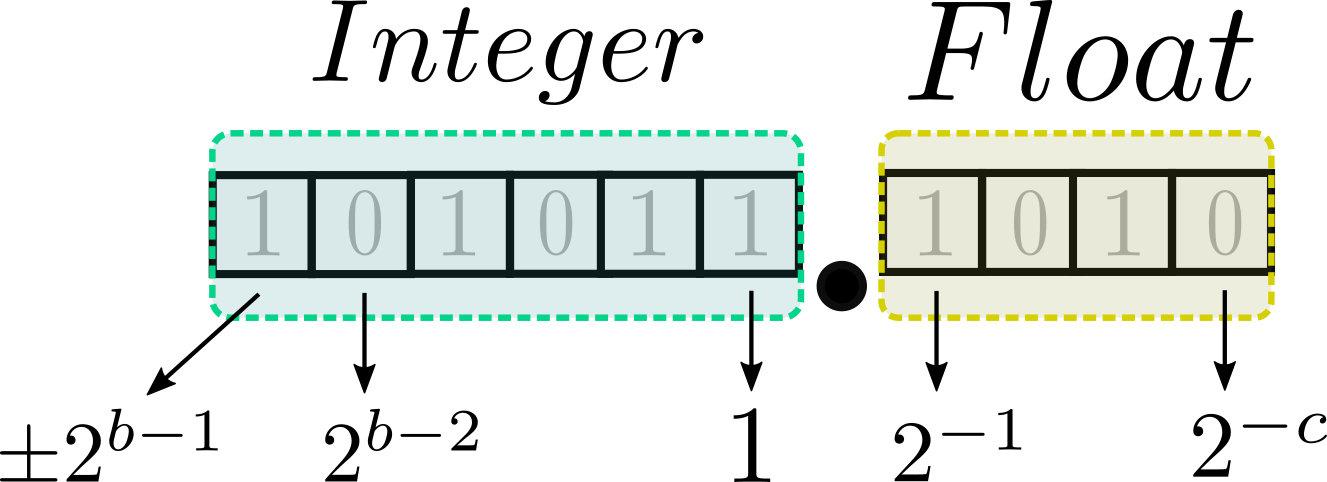
\includegraphics[scale=1]{data/bits.png}
  \par\end{centering}
  \caption{View of the value of each bit}
\end{figure}
As lowest significant bit worths $2^{-c}$ then the resolution is $2^{-c}$ and this works in both signed and unsigned cases
\\
Thought, to compute the range we need to separate in two cases, looking at which is the greater (we call it $r$) and the lower (we call it $l$) number in each case.
In the unsgined case the lower number is 0 and the highest will be
$$r=\underbrace{2^{-c}+2^{-c+1}+...+2^{-1}}_{1-2^{-c}}+\underbrace{1+2^{1}+...+2^{b-1}}_{2^{b}-1}=2^{b}-2^{-c}$$
So the resolution is just $r-l=2^{b}-2^{-c}$
\\
With the signed case we note the smallest number is when only most significant bit is 1
$$l=-2^{b-1} $$
And the highest when all bits are 1 except the most significant one
$$r=2^{-c}+2^{-c+1}+...+2^{1}+1+2^{1}+...+2^{b-2}=2^{b-1}-2^{-c}$$
Thus the resolution is $r-l=2^{b-1}-2^{-c}+2^{b-1}=2^{b}-2^{-c}$
That is the same, that is reasonable because we can express the same amount of numbers with the same amount of bits and that doesn't depend on whether the number is signed or not

